\subsection{Overview}

\textit{CLAN} (Closely reLated ApplicatioNs) \cite{McMillan:2012:DSS:2337223.2337267} is an approach for automatically detecting similar Java applications by exploiting the semantic layers corresponding to packages class hierarchies. \textit{CLAN} works based on the document framework for computing similarity, semantic anchors, e.g. those that define the documents' semantic features. Semantic anchors and dependencies help obtain a more precise value for similarity computation between documents. The assumption is that if two applications have API calls implementing requirements described by the same abstraction, then the two applications are more similar than those that do not have common API calls. The approach uses API calls as semantic anchors to compute application similarity since API calls contain precisely defined semantics. The similarity between applications is computed by matching the semantics already expressed in the API calls.

\subsection{The Approach}

The process consist of 12 steps here graphically reported.

\begin{figure}[H]
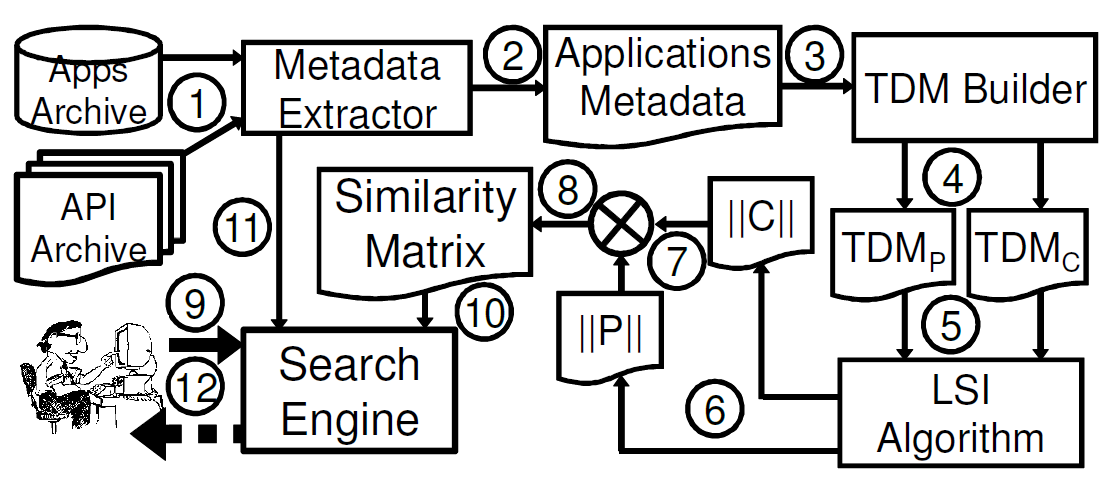
\includegraphics[width=15cm,height=20cm,keepaspectratio]{images/Clan.png}
\centering
\caption{CLAN phases.}
\end{figure}

\subsubsection{1 - 3: Terms Extraction}
Steps from 1 to 3 can be merged together since are related to extraction of terms from the repositories.
As stated before, an important concept is that terms extracted are only API calls, this means that all other things present in a piece of code are discarded, for example all the variables or the function declaration and invocation. Furthermore these API calls belong only to the JDK, in such a way also the calls to any other external library are discarded. This idea is also applied in the extraction of the import declaration, focus only on the JDK packages import.
The result of this process will be an ordered set of data, representing the occurrencies of any Package;Class for all the projects.

\subsubsection{4: TDMs Creation}
Once the dataset as been created, is reorganized in TDMs. Here two different matrices are created, one for the Classes and one for the Packages. Class-level and package-level similarities are different since applications are often more similar on the package level than on the class level because there are fewer packages than classes in the JDK. Therefore, there is the higher probability that two applications may have API calls that are located in the same package but not in the same class.

\subsubsection{5: LSI Procedure}

\subsubsection{6: Apply the Cosine Similarity}

\subsubsection{7: Sum of the matrices}
The 2 matrices are summed, but before are multplied by a certain value. Since the values for the entries in the 2 matrices are between 0.0 and 1.0 a simple sum could result in a value over 1.0, by this multiplication these values are reducted in order to be summed togheter but still maintaining the logical meaning. The authors chosen 0.5, also we, since is a good value to equal distribute the weight of the packages and method calls.The sum of this value is 1.0, and can span from 0.1 to 0.9 for each matrix, is clear that more is high on a matrix, more is important the values that we are considering from such matrix.

\subsubsection{8: Final similarity matrix}